\documentclass[10pt,onecolumn,letterpaper]{article}
%% Welcome to Overleaf!
%% If this is your first time using LaTeX, it might be worth going through this brief presentation:
%% https://www.overleaf.com/latex/learn/free-online-introduction-to-latex-part-1

%% Researchers have been using LaTeX for decades to typeset their papers, producing beautiful, crisp documents in the process. By learning LaTeX, you are effectively following in their footsteps, and learning a highly valuable skill!

%% The \usepackage commands below can be thought of as analogous to importing libraries into Python, for instance. We've pre-formatted this for you, so you can skip right ahead to the title below.

%% Language and font encodings
\usepackage[spanish,english]{babel}
\usepackage[utf8x]{inputenc}
\usepackage[T1]{fontenc}

%% Sets page size and margins
\usepackage[a4paper,top=3cm,bottom=2cm,left=3cm,right=3cm,marginparwidth=1.75cm]{geometry}

%% Useful packages
\usepackage{amsmath}
\usepackage{graphicx}
\usepackage[colorinlistoftodos]{todonotes}
\usepackage[colorlinks=true, allcolors=blue]{hyperref}

%% Title
\title{
		%\vspace{-1in} 	
		\usefont{OT1}{bch}{b}{n}
		\normalfont \normalsize \textsc{MIE 1624 Introduction to Data Science and Analytics} \\ [10pt]
		\huge Assignment 2: Ordinal Logistic Regression \\
}

\usepackage{authblk}

\author{Yunjie Xu 1008601951}


	\affil{\small{Department of Mechanical and Industrial Engineering, University of Toronto}}


\begin{document}
\maketitle

\selectlanguage{english}


%%\begin{abstract}
%%The abstract is probably what you'll be writing last, and should be roughly 300 words in length. Your abstract will get published whether or not your team wins the challenge, so make sure to do an extra good job of it! An easy way to structure your abstract is to write individual summaries of the four parts of your paper (Introduction, Methods, Results, Discussion) and then put them together once you're done.
%%\end{abstract} \\ 
%%\\ 
%%{\textbf{Keywords} \\
%%pick, 3-5, good, keywords}

\section*{Introduction}
For this assignment, the aims are to train, validate, and tune multi-class ordinary classification models that can classify the respondent's annual salary in which range based on the kaggle\_survey\_2022\_responses.csv dataset.


\section*{Part 1}
Firstly, I checked the duration of time for each respondent, and I didn't find any possible invalid questionnaires. Secondly, I dropped the option "OTHER" because that option was pretty vague, and I filled 0 with NaN values and replaced the string with 1 in multiple-choice questions. I didn't combine multiple-choice questions because there is no evidence to show that every language, method, or platform is equally important. Thus, treating each part of multiple choice questions as an independent question was more conformed to reality. Thirdly, I classified the rest of the questions into ordinal variables and nominal variables, and then I treaded nominal variables with pd.get\_dummies and ordinal variables with numerical encode. Fourth is dealing with missing values. I deleted questions if more than 1/3 of the values were missing. And I imputed the rest of the missing values using the KNN classifier. The final step was encoding the target value, and I moved the target column(Q25\_Encoded ) to the rightmost.

\section*{Part 2}
\subsection*{Exploratory data analysis}
I first explored the distributions of the participants’ countries of origin, coding experiences, and salary range distributions. It is found that India and the United States are the two major countries survey participants came from; most participants have 1-3 years of coding experience. There are 15 different classes in the target value, but more than 1/3 of respondents were classified into class 0, whose salary range is below 10000 (Figure 1).

\subsection*{Feature Selection}
I used two ways in feature selection. One is the correlation, and another is Mutual Information. For the correlation method, I plotted correlation plot first(Figure 2), then I selected the top 50 features most correlated to the target value(Figure 3). Then I used recursive feature elimination to choose the top 40 features that are more or most relevant in predicting the target variable(Figure 4). Mutual Information is calculated between two variables and measures the reduction in uncertainty for one variable given a known value of the other variable. Thus, I used mutual\_info\_classif to select the top 40 features(Figure 5). The results are basically the same by two different methods, with only a few less important factors being different. Thus, I used the result from the second method to do the following analysis

\section*{Part 3}
 I defined a function to implement ordinal logistic regression and validated it using a 10-folder cross-validation, because the response has 15 levels, thus I cannot fit a single Logistic regression that only classifies a binary class response. Therefore, my function defined could did 14 times binary classifications from the lowest class to the highest class.\\ \\
 I first created an empty list to store the probabilities to return and set the initial probability to 0. Then, I created a while loop that, while the iterations are less than 13, classifies 0 and 1 based on y\_train, and trained the Logistic regression based on the classification through the scikit-learn library. I predicted the probability of class 0 for the current iteration based on X\_val, appended the probability to the list we created in the beginning, p\_list, and then updated the initial probability. Thus, now it was the probability of 0 up to the current level and continued with another iteration. When it iterated 14 times, the function appended the probability of class “1” to the p\_list. Now the model is trained, and all possibilities are returned. p\_list is a 2-d array, and each row has 15 elements which represent the probability from class 0 to class 14, and the number of rows equaled with the numbers in each fold.\\\\
 I implemented the algorithm on a 10-fold cross-validation. And I used some code provided by our class. The average accuracy is 37.669\%, with the standard deviation of 4.371\%.\\\\
 I calculated the bias based on MSE and variance. Then I fitted multiple models with different C, the model complexity, and found the bias and variance each time to explain C values effects on the model performance. The results are as expected. And I plotted the bias-variance trade-off (Figure 6) for the different C values graph. As model complexity increases, bias decreases, and variance increases. The best model appears to be somewhere around when bias and variance interact with each other.  


\section*{Part 4}
The ordinal logistic regression contains the following hyperparameters: ‘penalty’, ’dual’, ‘tol’, ‘C’, ‘fit\_intercept’, ‘intercept\_scaling’, ‘class\_we ight’, ‘random\_state’, ‘solver’, ‘max\_iter’, ‘multi\_class ’, ‘verbose’, ‘warm\_start’, ‘n\_jobs’, ‘l1\_ratio’.  I tuned C and solver hyperparameters. The steps were basically the same as the last part. But there were more different models that needed to be tried here. I tried C values from 0.00001 to 0.01, and solver type 'newton-cg', 'liblinear','lbfgs',  'sag'. From the results, the best parameters were  ‘C’ is 10 and ‘solver’ is ‘lbfgs'. The highest accuracy is 39.392\%(1.863\%), the best F1 score is 0.14\%(0.011\%), and the best Recall is 0.137\%(0.0\%).\\\\
In sklearn, C equals with $C=\frac{1}{\lambda}$,the smaller C means the heavier penalty and the stronger the regularization effect will be. C = 100 here means here is nearly no need for penalty term\\\\
I used both accuracy and F1 score to examine the model performance. The first reason is that accuracy is a straightforward way to see how the model performs. It tells us how many observations are correctly classified. Secondly, the F1 score is also essential since the observation scale is small, but 15 classes need to be classified.So if we have metrics recall and precision, we can get the proportion of observations correctly classified and the proportion of wrongly classified observations. We can get a balance of two using F1 score. And accuracy cannot be a suitable performance metric for this problem. Therefore, I used F1 score as the examination of model performance.\\\\
I plotted the important features(Figure 7), and I found feature importance changed a lot compared with the plot in section 2. Only the location factor(Q4) was still very important. Other important factors had changed a lot. Thus, I think the location factor(Q4) is the most important feature in this dataset, which means data worker can also earn more if they live in higher-income country.

\section*{Part 5}
I applied the algorithm to the test set and got the predicted probabilities of each observation belonging to each class for the test set, and classified the observations into classes based on these probabilities. The accuracy on test set is 39.256\%,  and the F1 score is 0.117. Finally, I plotted the model performance on classes(Figure 8,Figure 9). \\\\

In my opinion, this dataset is underfitting. The main reason is the scale of observations is too small. I need more observations. Another reason is the unbalance of the distribution of target values, which further exacerbates the underfitting situation. For example, most target values are concentrated at class 0, and only a few observations are classified into the rest of class. Thirdly, I had to separate the training, testing, and validation set, which also made fitting worse. Thus, this assignment's core problem is that the data size is too small, and there are too many categories in the target columns. If we would like to increase accuracy, I suggest decreasing the weight of class 0 when we train the model, by half, for example. I would allocate more weight to the other classes and be more likely to classify the class other than 0.

\section*{Appendix}

\appendix

\begin{figure}[htbp]
  \centering
  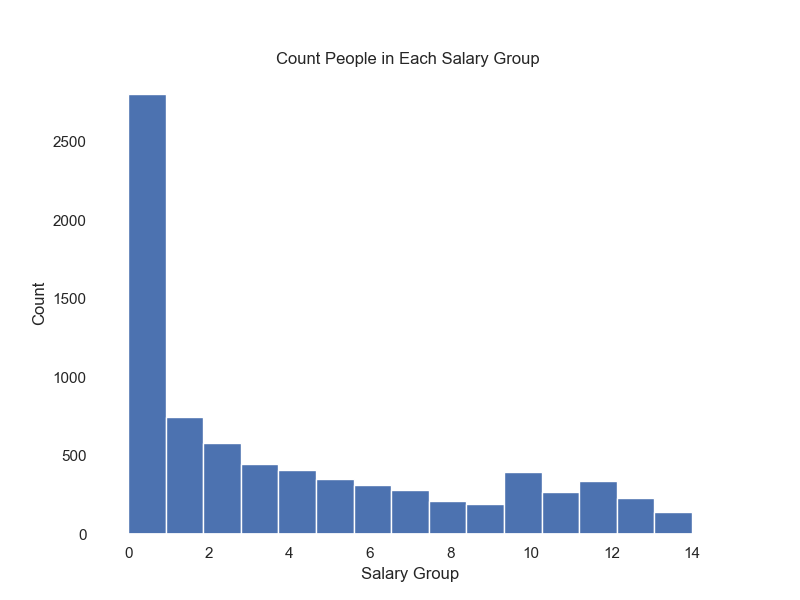
\includegraphics[width=.75\textwidth]{f1.png}
  \caption{Count People in Each Salary Group}
\end{figure}

\begin{figure}[htbp]
  \centering
  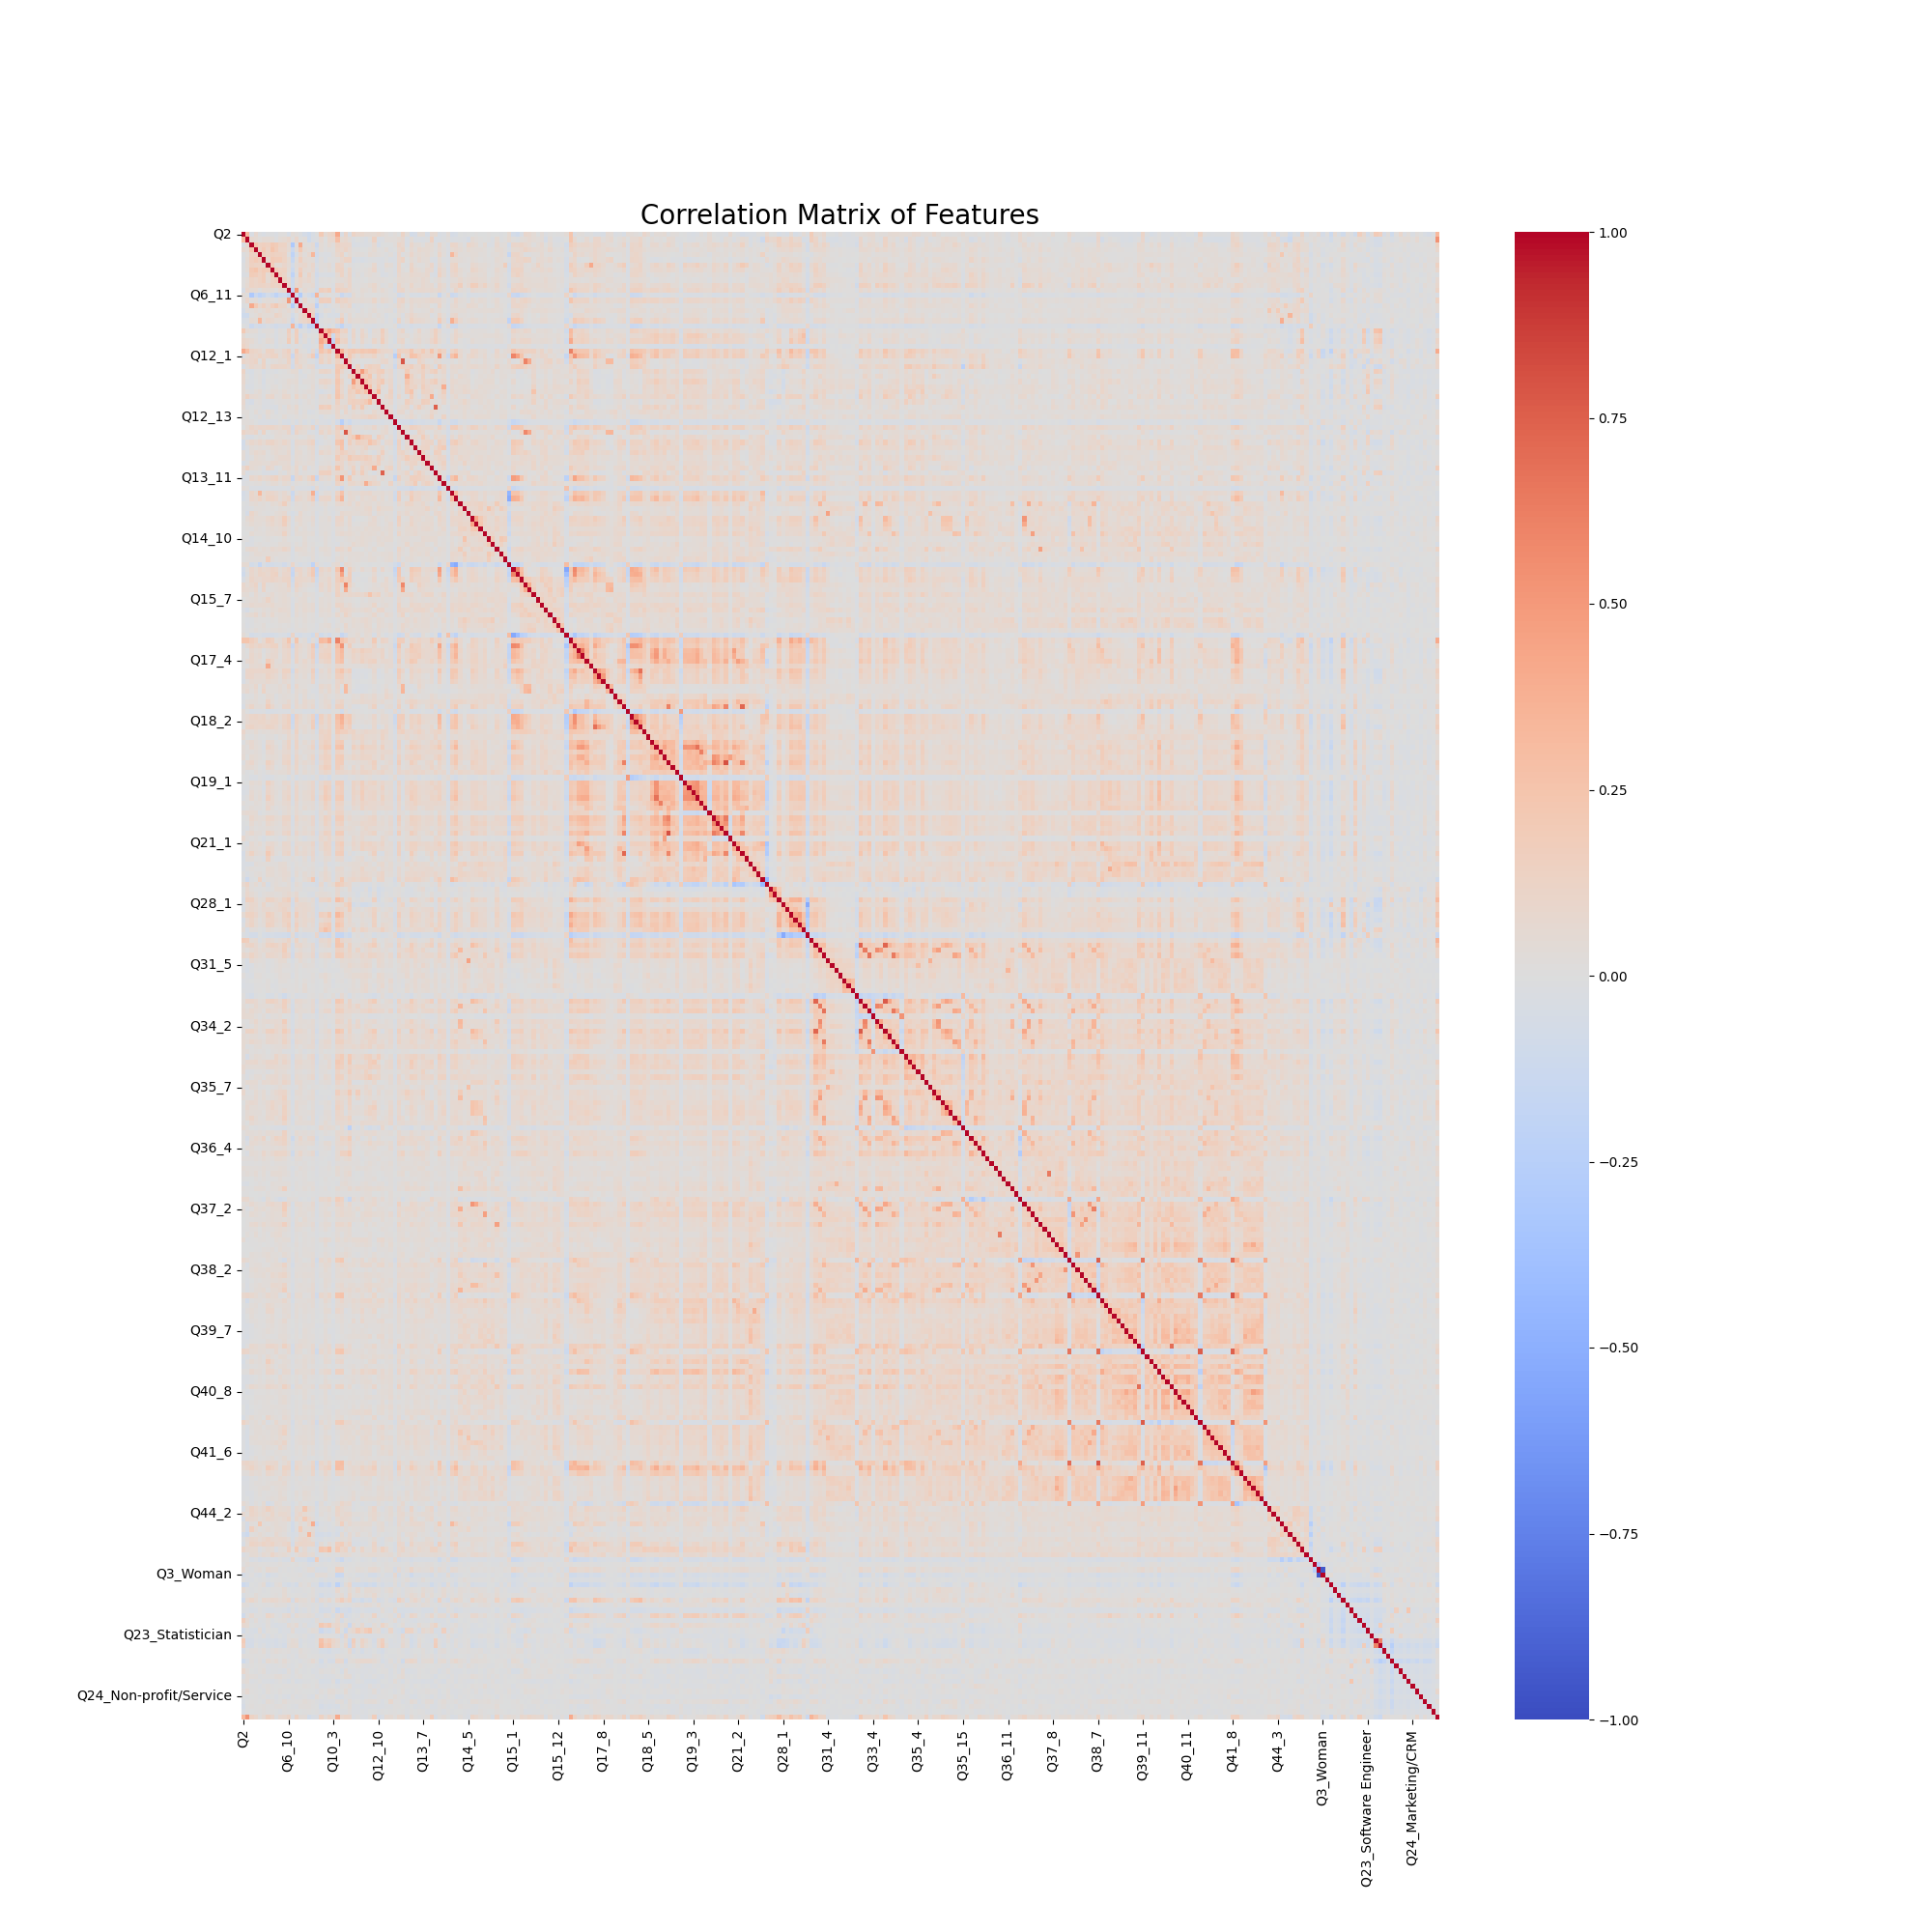
\includegraphics[width=.75\textwidth]{f2.png}
  \caption{Correlation Matrix of Features}
\end{figure}

\begin{figure}[htbp]
  \centering
  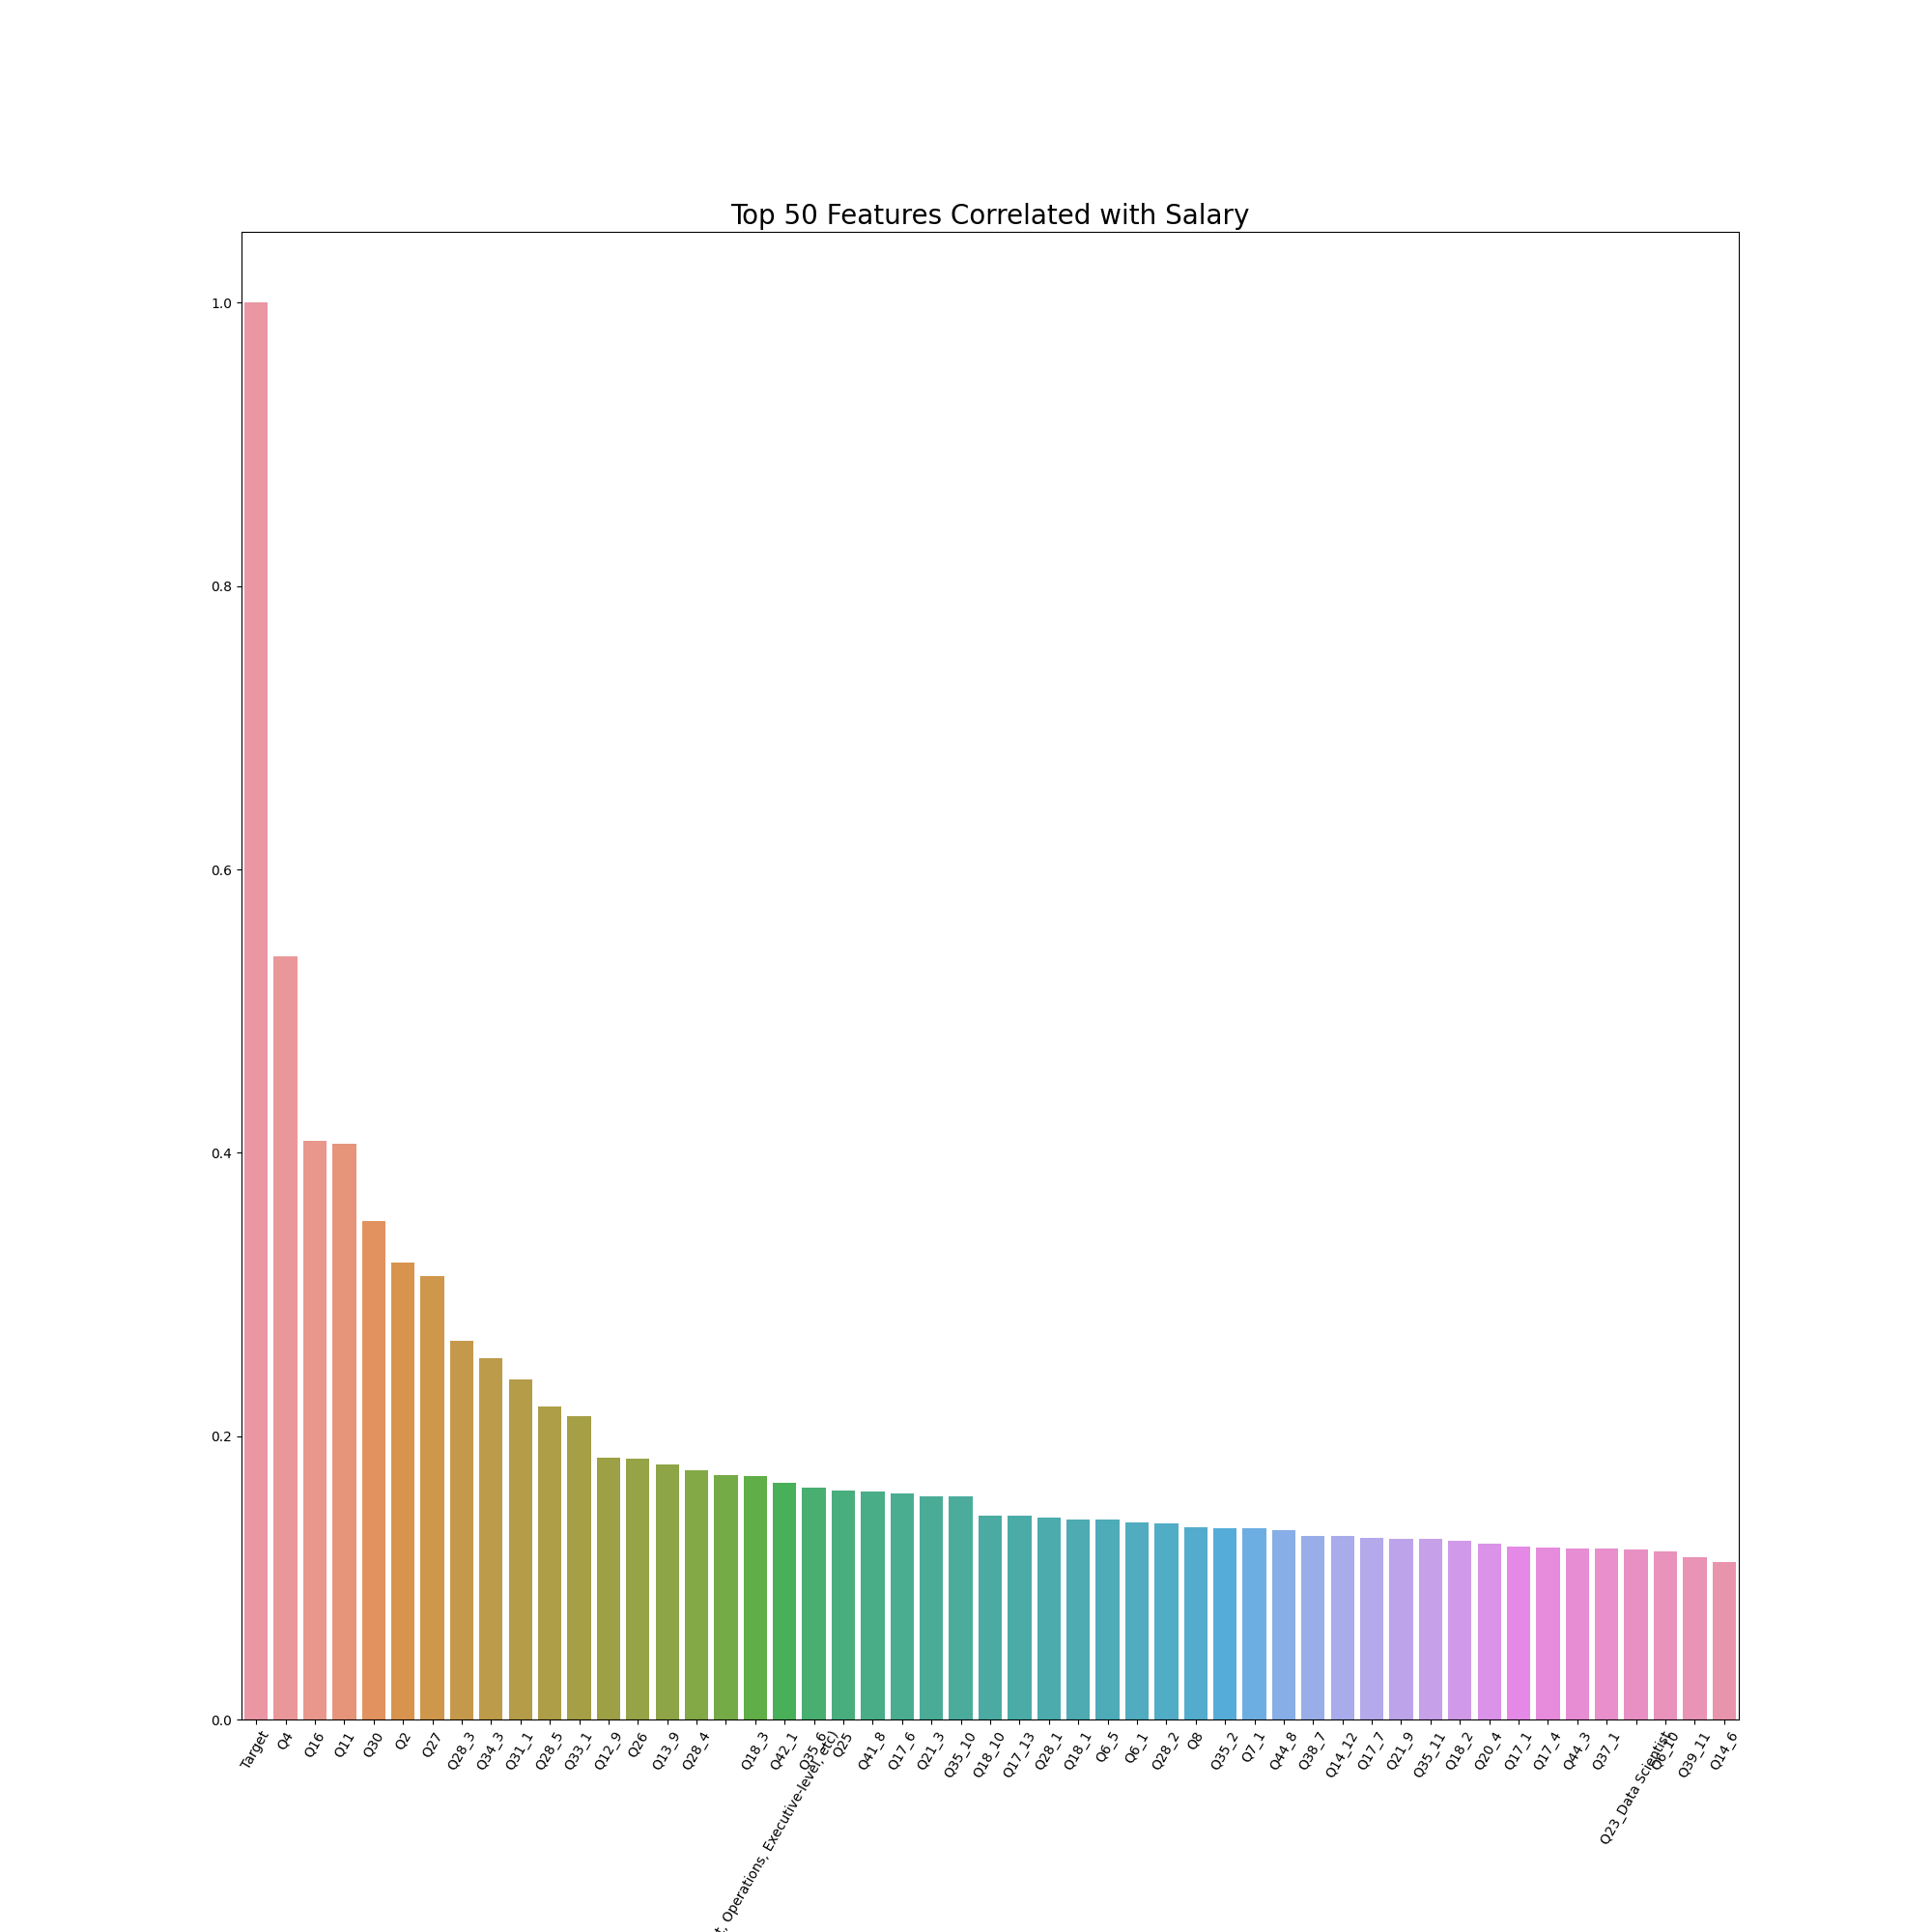
\includegraphics[width=.75\textwidth]{f3.png}
  \caption{Top 50 Features Correlated with Salary}
\end{figure}

\begin{figure}[htbp]
  \centering
  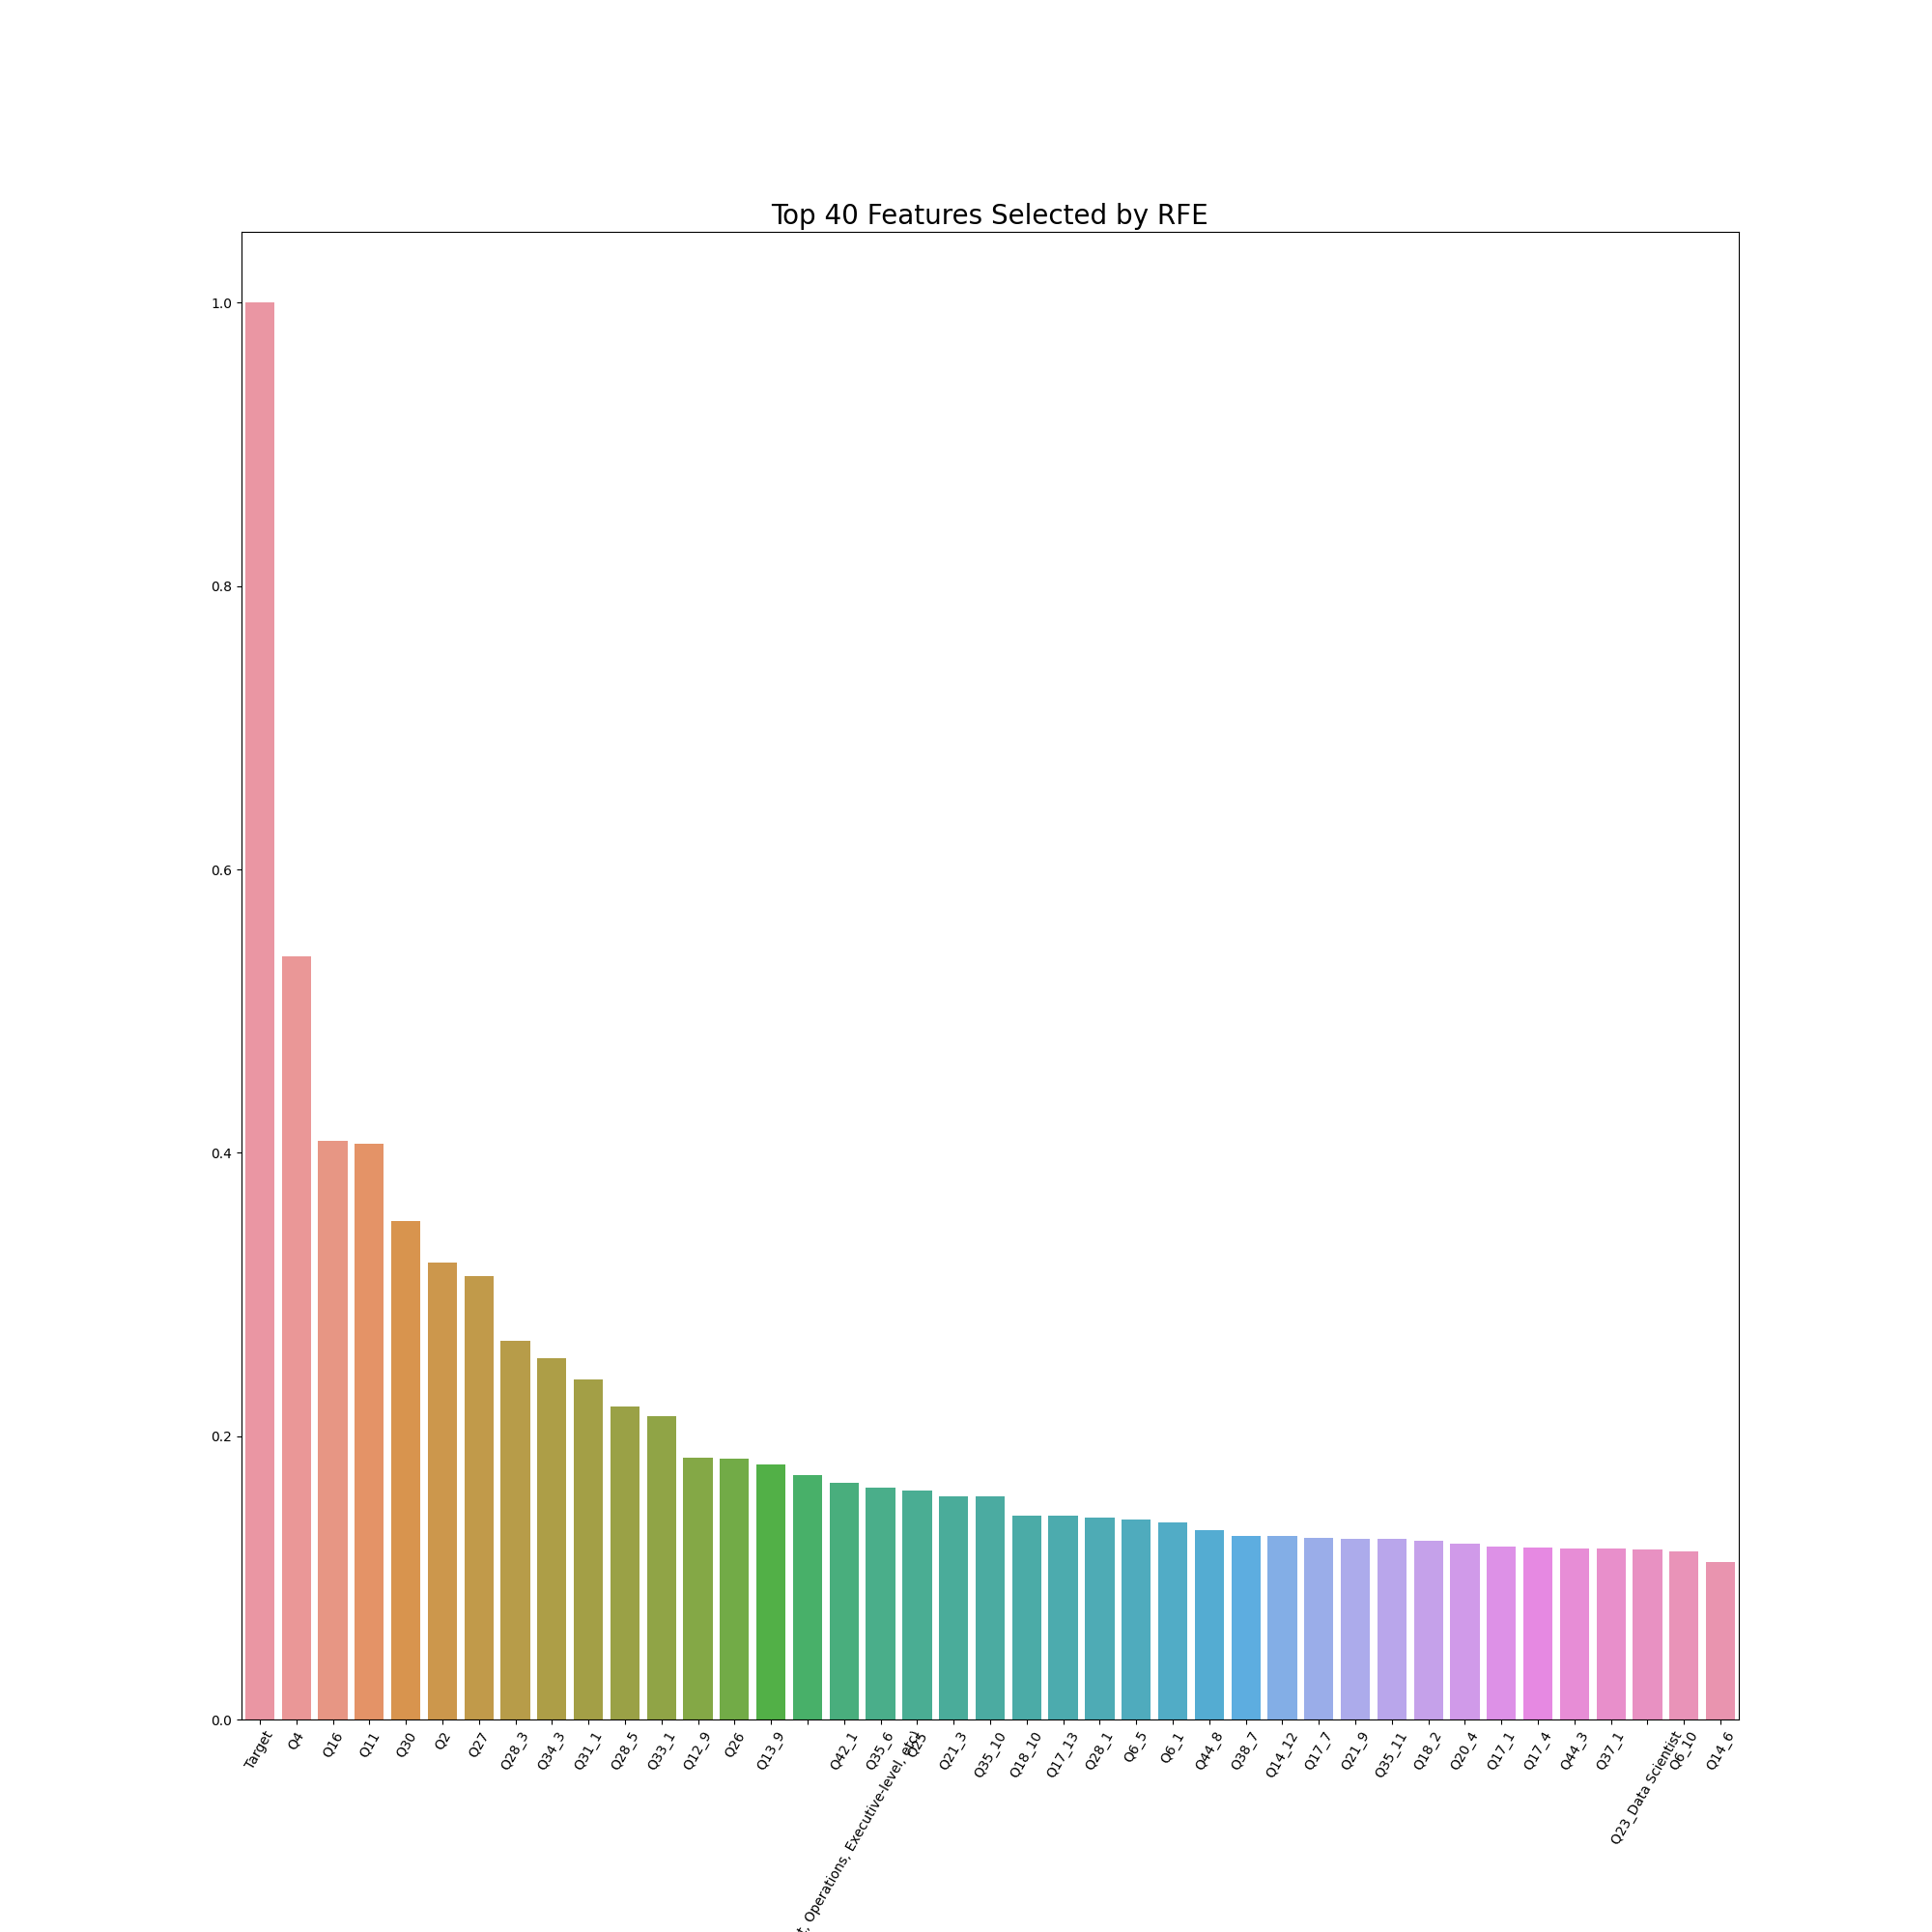
\includegraphics[width=.75\textwidth]{f4.png}
  \caption{Top 40 Features Selected by RFE}
\end{figure}

\begin{figure}[htbp]
  \centering
  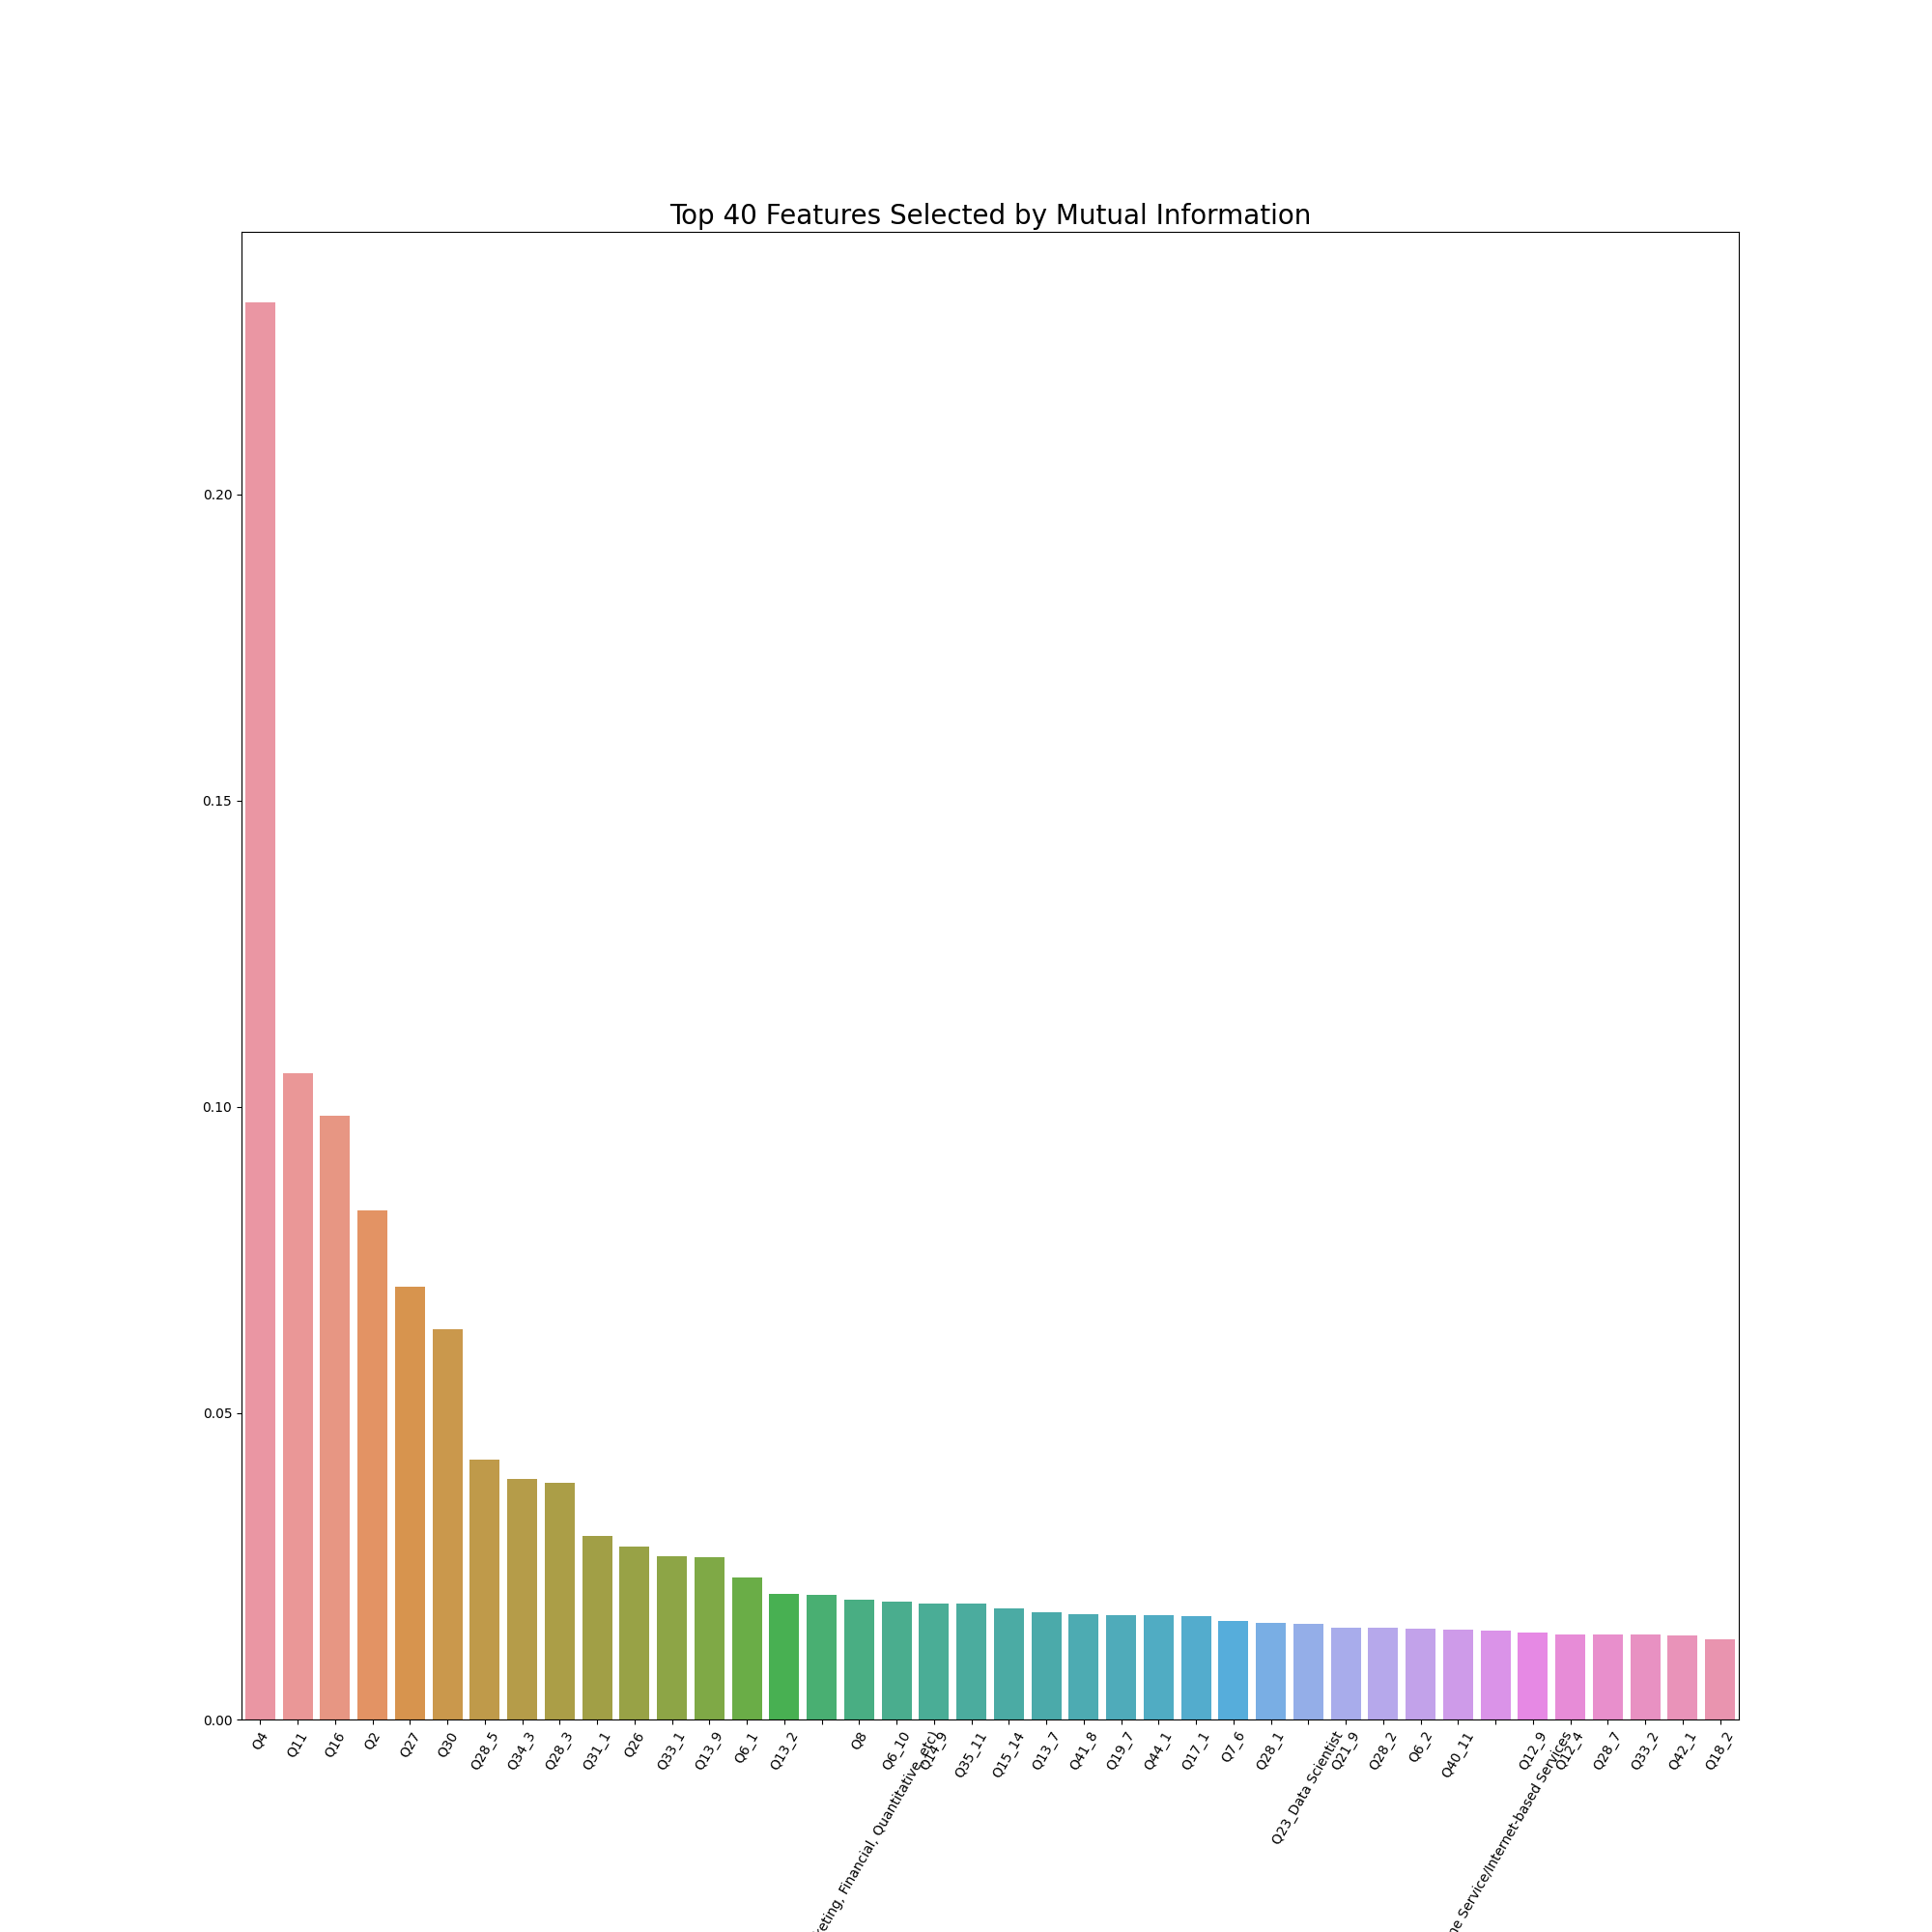
\includegraphics[width=.75\textwidth]{f25.png}
  \caption{Top 40 Features Selected by Mutual Information}
\end{figure}

\begin{figure}[htbp]
  \centering
  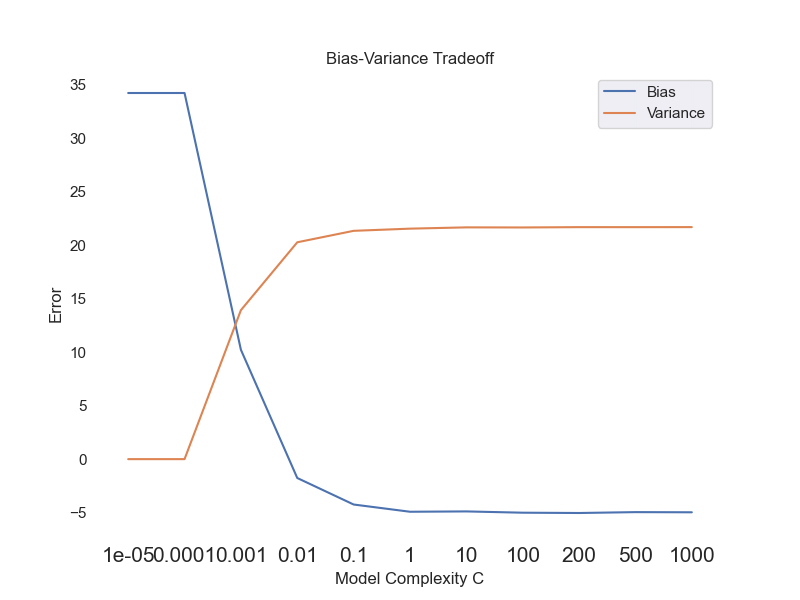
\includegraphics[width=.75\textwidth]{f6.png}
  \caption{Bias-Variance Tradeoff}
\end{figure}

\begin{figure}[htbp]
  \centering
  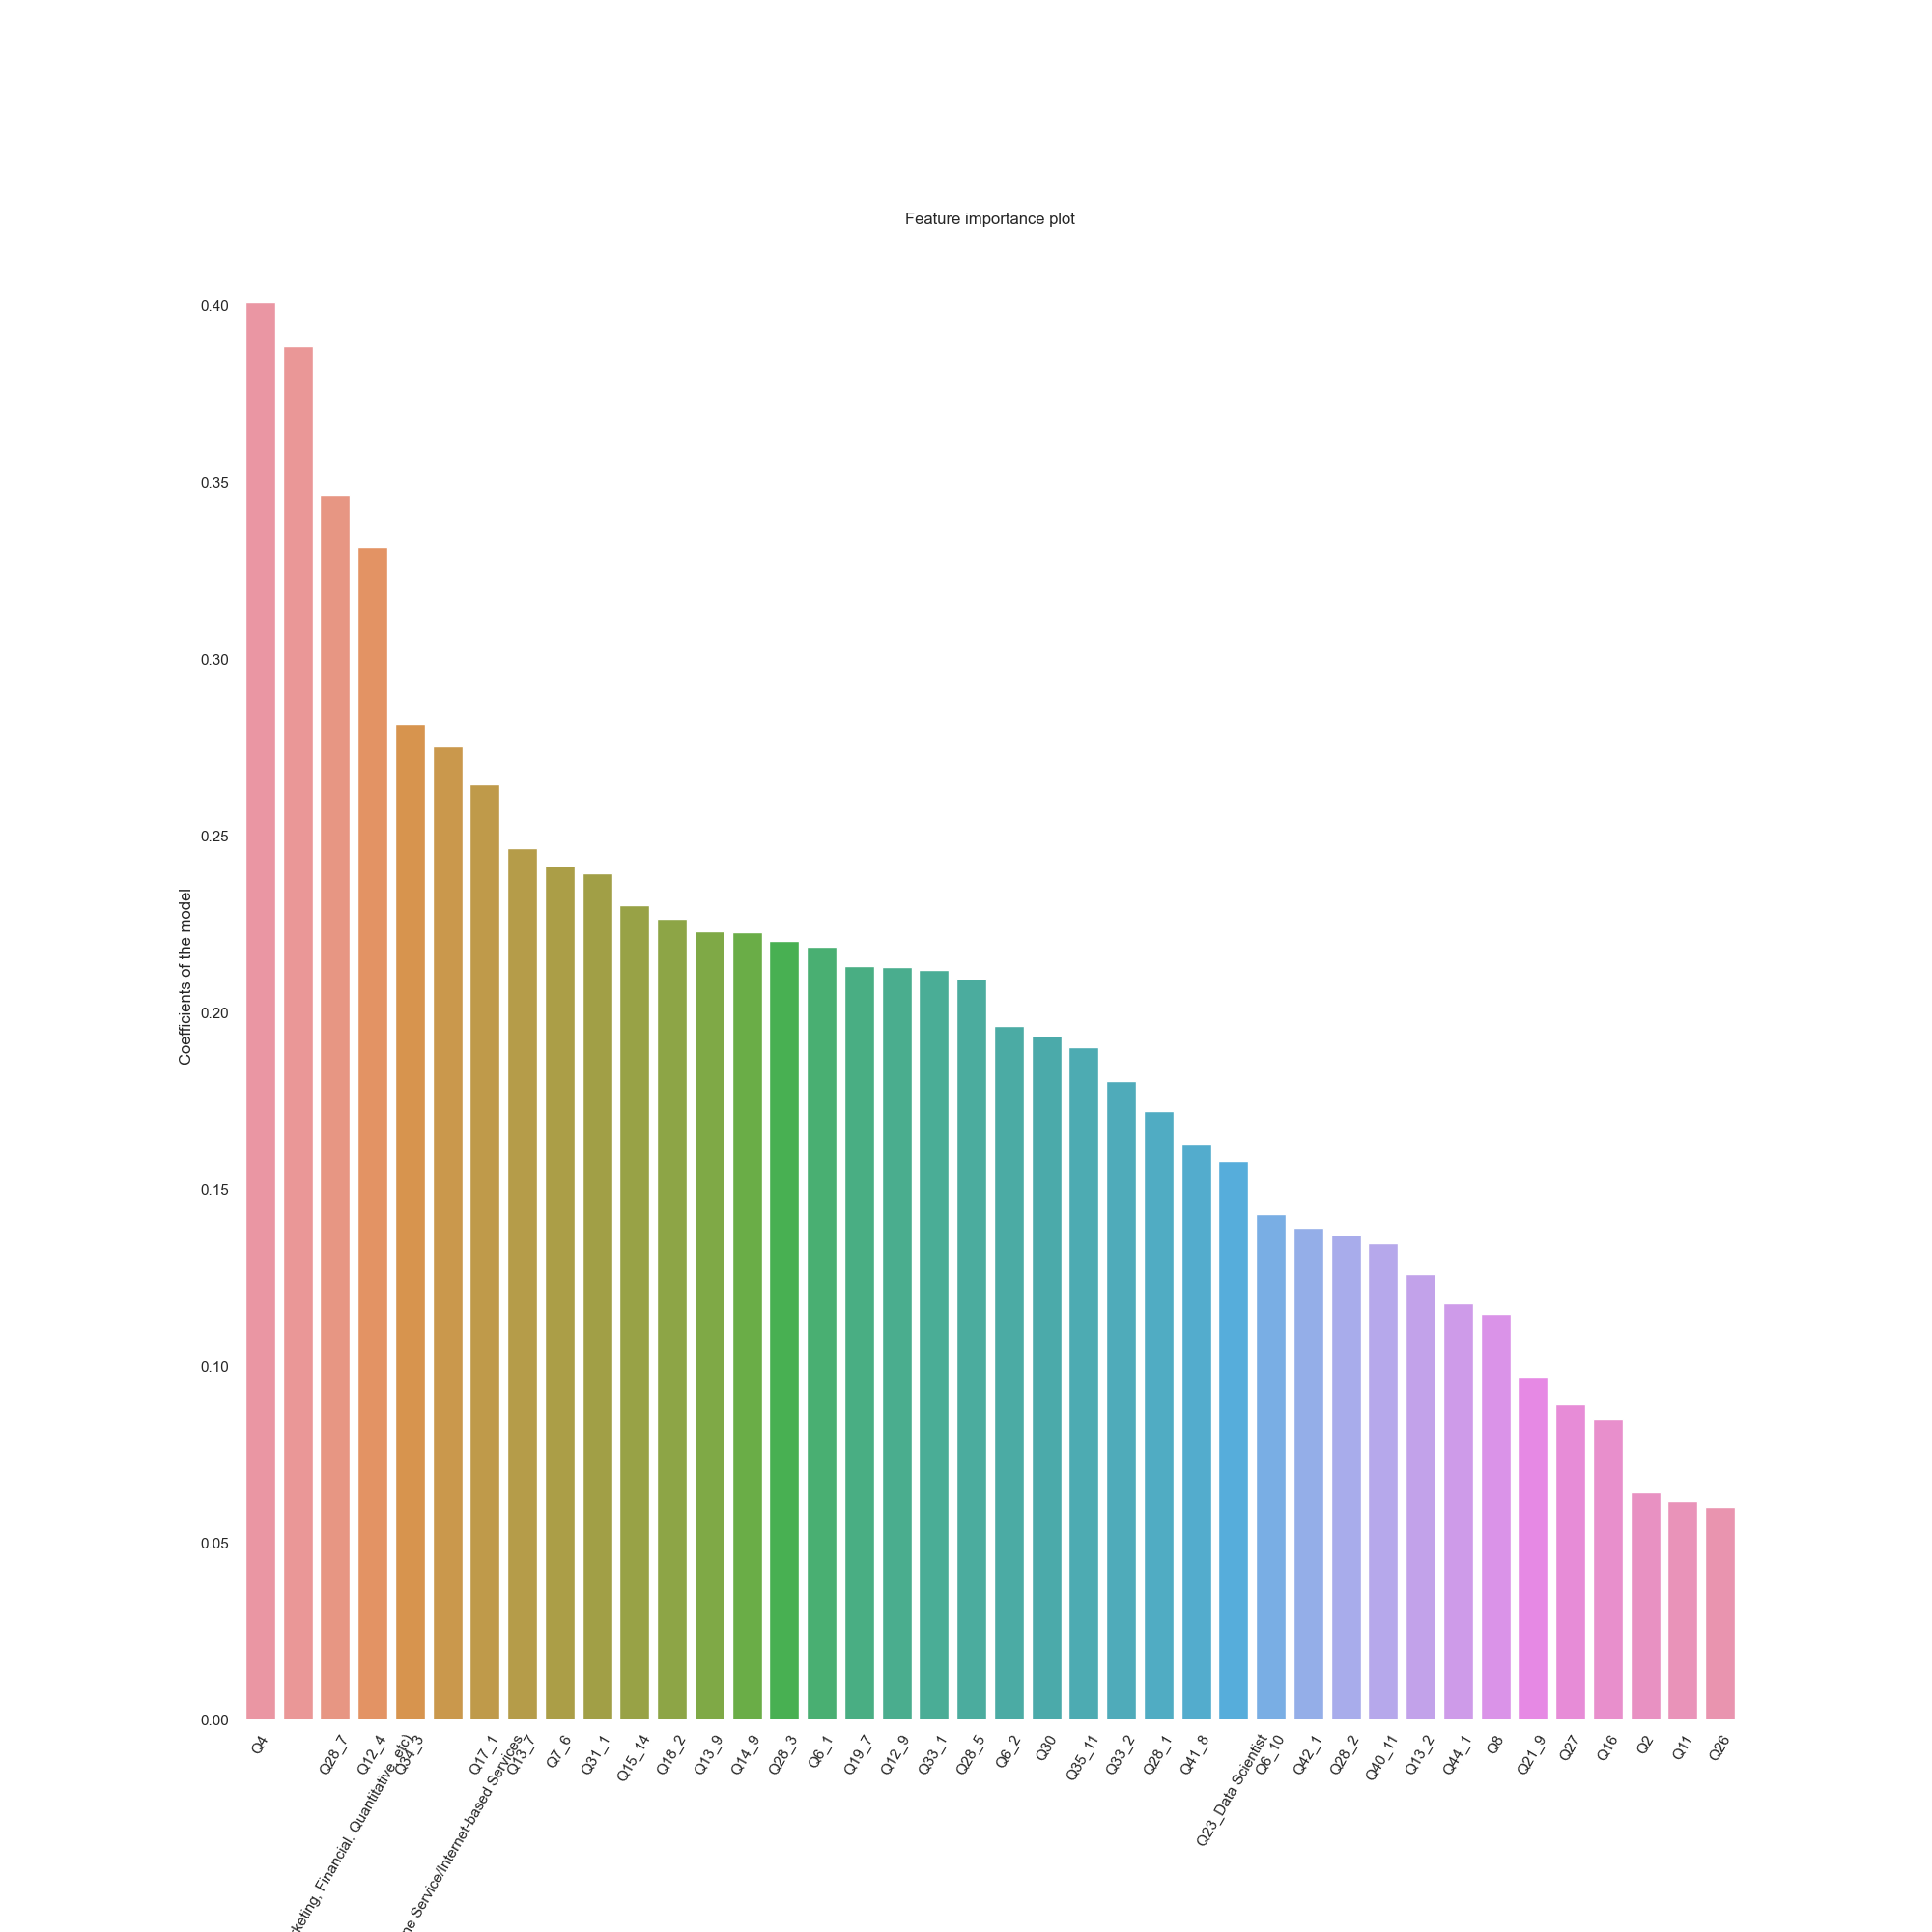
\includegraphics[width=.75\textwidth]{f7.png}
  \caption{Feature importance plot in Part 4}
\end{figure}

\begin{figure}[htbp]
  \centering
  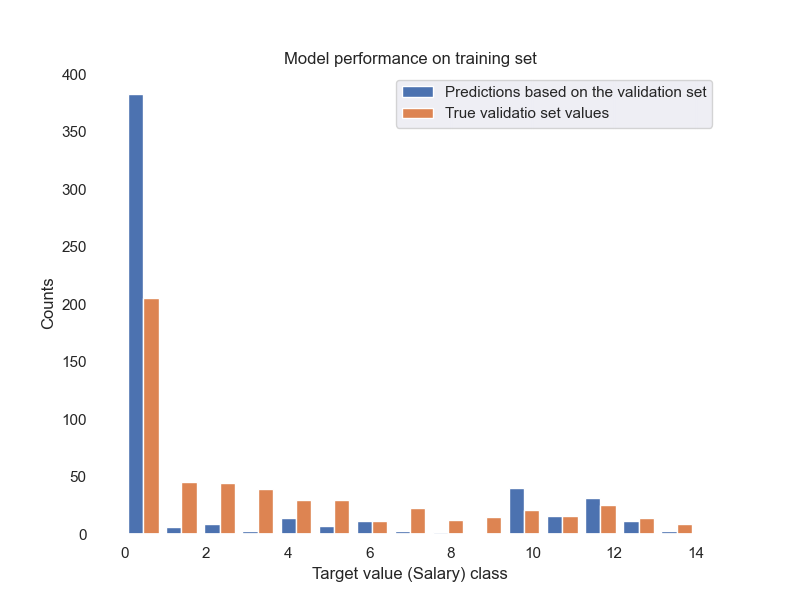
\includegraphics[width=.75\textwidth]{f8.png}
  \caption{Model performance on validation set}
\end{figure}

\begin{figure}[htbp]
  \centering
  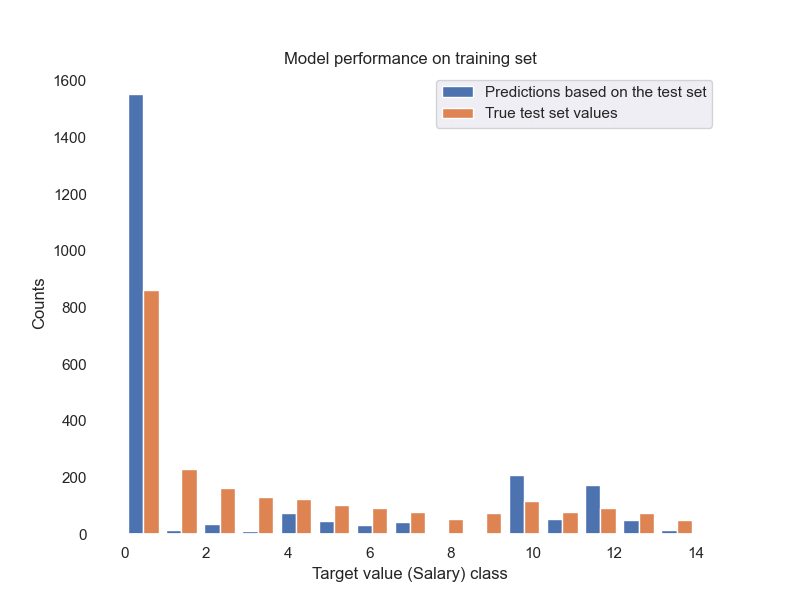
\includegraphics[width=.75\textwidth]{f9.png}
  \caption{Model performance on training set}
\end{figure}

\end{document}